\documentclass[a4paper,12pt]{extarticle}
\usepackage[utf8x]{inputenc}
\usepackage[T1,T2A]{fontenc}
\usepackage[russian]{babel}
\usepackage{hyperref}
\usepackage{indentfirst}
\usepackage{listings}
\usepackage{color}
\usepackage{here}
\usepackage{array}
\usepackage{multirow}
\usepackage{graphicx}

\usepackage{caption}
\renewcommand{\lstlistingname}{Программа} % заголовок листингов кода

\bibliographystyle{ugost2008ls}

\usepackage{listings}
\lstset{ %
extendedchars=\true,
keepspaces=true,
language=C,						% choose the language of the code
basicstyle=\footnotesize,		% the size of the fonts that are used for the code
numbers=left,					% where to put the line-numbers
numberstyle=\footnotesize,		% the size of the fonts that are used for the line-numbers
stepnumber=1,					% the step between two line-numbers. If it is 1 each line will be numbered
numbersep=5pt,					% how far the line-numbers are from the code
backgroundcolor=\color{white},	% choose the background color. You must add \usepackage{color}
showspaces=false				% show spaces adding particular underscores
showstringspaces=false,			% underline spaces within strings
showtabs=false,					% show tabs within strings adding particular underscores
frame=single,           		% adds a frame around the code
tabsize=2,						% sets default tabsize to 2 spaces
captionpos=t,					% sets the caption-position to top
breaklines=true,				% sets automatic line breaking
breakatwhitespace=false,		% sets if automatic breaks should only happen at whitespace
escapeinside={\%*}{*)},			% if you want to add a comment within your code
postbreak=\raisebox{0ex}[0ex][0ex]{\ensuremath{\color{red}\hookrightarrow\space}},
texcl=true,
inputpath=listings,                     % директория с листингами
}

\usepackage[left=2cm,right=2cm,
top=2cm,bottom=2cm,bindingoffset=0cm]{geometry}

%% Нумерация картинок по секциям
\usepackage{chngcntr}
\counterwithin{figure}{section}
\counterwithin{table}{section}

%%Точки нумерации заголовков
\usepackage{titlesec}
\titlelabel{\thetitle.\quad}
\usepackage[dotinlabels]{titletoc}

%% Оформления подписи рисунка
\addto\captionsrussian{\renewcommand{\figurename}{Рисунок}}
\captionsetup[figure]{labelsep = period}

%% Подпись таблицы
\DeclareCaptionFormat{hfillstart}{\hfill#1#2#3\par}
\captionsetup[table]{format=hfillstart,labelsep=newline,justification=centering,skip=-10pt,textfont=bf}

%% Путь к каталогу с рисунками
\graphicspath{{fig/}}

%% Внесение titlepage в учёт счётчика страниц
\makeatletter
\renewenvironment{titlepage} {
 \thispagestyle{empty}
}
\makeatother


\begin{document}	% начало документа

% Титульная страница
\begin{titlepage}	% начало титульной страницы

	\begin{center}		% выравнивание по центру

		\large Санкт-Петербургский Политехнический Университет Петра Великого\\
		\large Институт компьютерных наук и технологий \\
		\large Кафедра компьютерных систем и программных технологий\\[6cm]
		% название института, затем отступ 6см
		
		\huge Базы данных\\[0.5cm] % название работы, затем отступ 0,5см
		\large Отчет по лабораторной работе №1\\[0.1cm]
		\large Разработка структуры БД\\[5cm]

	\end{center}


	\begin{flushright} % выравнивание по правому краю
		\begin{minipage}{0.25\textwidth} % врезка в половину ширины текста
			\begin{flushleft} % выровнять её содержимое по левому краю

				\large\textbf{Работу выполнил:}\\
				\large Графов Д.И.\\
				\large {Группа:} 33531/2\\
				
				\large \textbf{Преподаватель:}\\
				\large Мяснов А.В.

			\end{flushleft}
		\end{minipage}
	\end{flushright}
	
	\vfill % заполнить всё доступное ниже пространство

	\begin{center}
	\large Санкт-Петербург\\
	\large \the\year % вывести дату
	\end{center} % закончить выравнивание по центру

\thispagestyle{empty} % не нумеровать страницу
\end{titlepage} % конец титульной страницы

\vfill % заполнить всё доступное ниже пространство


% Содержание
% Содержание
\renewcommand\contentsname{\centerline{Содержание}}
\tableofcontents
\newpage




\section{Цель работы}
Познакомить студентов с языком создания запросов управления данными SQL-DML.

\section{Программа работы}
\begin{itemize}
	\item Изучение SQL-DML.
	\item Выполнение всех запросов из списка стандартных запросов. Демонстрация результатов преподавателю.
	\item Получение у преподавателя и реализация SQL-запросов в соответствии с индивидуальным заданием. Демонстрация результатов преподавателю.
	\item Сохранение в БД выполненных запросов SELECT в виде представлений, запросов INSERT, UPDATE или DELETE -- в виде ХП. Выкладывание скрипта в GitLab.
\end{itemize}

\section{Теоретическая информация}
\large{EXPLAIN}
Cтруктура плана запроса представляет собой дерево узлов плана. Узлы на нижнем уровне дерева — это узлы сканирования, которые возвращают необработанные данные таблицы. Разным типам доступа к таблице соответствуют разные узлы: последовательное сканирование, сканирование индекса и сканирование битовой карты. Источниками строк могут быть не только таблицы, но и например, предложения VALUES и функции, возвращающие множества во FROM, и они представляются отдельными типами узлов сканирования. Если запрос требует объединения, агрегатных вычислений, сортировки или других операций с исходными строками, над узлами сканирования появляются узлы, обозначающие эти операции. И так как обычно операции могут выполняться разными способами, на этом уровне тоже могут быть узлы разных типов. В выводе команды EXPLAIN для каждого узла в дереве плана отводится одна строка, где показывается базовый тип узла плюс оценка стоимости выполнения данного узла, которую сделал для него планировщик. Если для узла выводятся дополнительные свойства, в вывод могут добавляться дополнительные строки, с отступом от основной информации узла. В самой первой строке (основной строке самого верхнего узла) выводится общая стоимость выполнения для всего плана; именно это значение планировщик старается минимизировать.

\section{Ход работы}
Каждая операция будет применена к одной таблице, так как для других выполнение
будет аналогично.

\subsection{Выполнение запросов из списка стандартных запросов}

\lstinputlisting[
	language=SQL,
	caption={common.sql},
]{../../src/common.sql}
\parindent=1cm % командна \lstinputlisting сбивает параментры отступа

Приведём некоторые примеры работы данного скрипта.
Со всеми примерами можно ознакомиться, запустив скрипт, расположенный в репозитории.

\href{http://gitlab.icc.spbstu.ru/grafa/wine_card}{http://gitlab.icc.spbstu.ru/grafa/wine\_card}

\newpage
\large{Результаты}

\begin{figure}[H]
	\begin{center}
		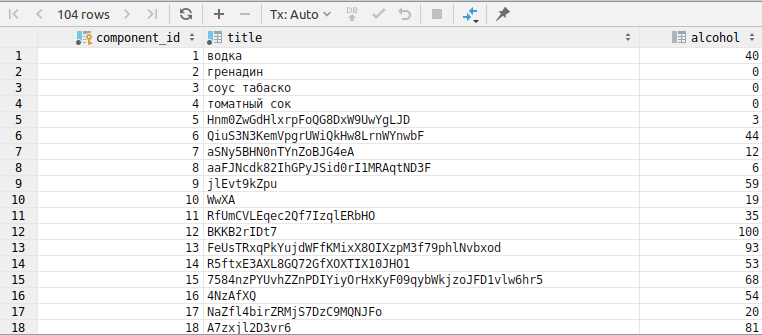
\includegraphics[scale=0.7]{1}
		\caption{Выборка всех данных из таблицы} 
		\label{pic:1} % название для ссылок внутри кода
	\end{center}
\end{figure}

\begin{figure}[H]
	\begin{center}
		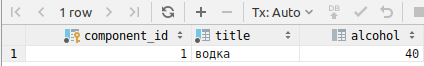
\includegraphics[scale=0.7]{2}
		\caption{Оператор LIKE} 
		\label{pic:2} % название для ссылок внутри кода
	\end{center}
\end{figure}

\begin{figure}[H]
	\begin{center}
		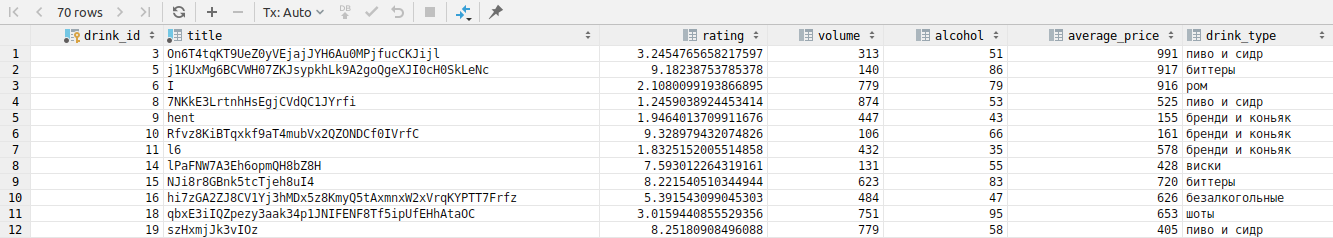
\includegraphics[scale=0.5]{4}
		\caption{Оператор BETWEEN} 
		\label{pic:4} % название для ссылок внутри кода
	\end{center}
\end{figure}

\begin{figure}[H]
	\begin{center}
		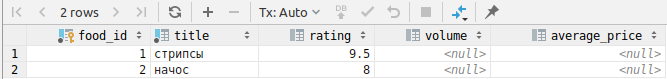
\includegraphics[scale=0.7]{5}
		\caption{Оператор IN} 
		\label{pic:5} % название для ссылок внутри кода
	\end{center}
\end{figure}

\subsection{Выполнение индивидуального задания}

Мной было получено индивидуальное задание, состоящее из 3 частей:
\begin{enumerate}
	\item Для каждого бара вывести топ-3 самых часто поставляемых за последний месяц единиц товара среди еды и напитков, рейтинг которых выше среднего по всем барам.
	\item Вывести перечень напитков, у которых количество ингредиентов для приготовления больше среднего. Отсортировать по уменьшению градуса.
	\item Для каждой акции вывести топ-3 напитков: самый крепкий алкогольный напиток, самый дешевый и самый большой по объему. Если для одной акции какие-то напитки в топ-3 совпадают, то выводить лишь один раз, без дублирования.
\end{enumerate}

Для всех запросов необходимо привести план запроса и пояснения.
\subsubsection{Индивидуальное задание №1}
Структурно запрос можно разделить на 2 части: первая вычисляет требуемую выборку для напитков, вторая -- для еды.
Рассмотрим работу одного из подзапросов:

С помощью оператора join мы формируем выборку из MANY-MANY таблицы supplies\_drinks и связанных с ней drinks и places. Затем c помощью оператора where ... and ... проводим фильтрацию по дате поставки (за последний месяц) и по рейтингу.

Затем вычисляем оконную функцию\\
\textit{row\_number() over (partition by p.place\_id order by d.drink\_id) top}\\
для подсчёта количества напитков в каждом заведении.\\
Далее из получившегося запроса делаем подзапрос и с помощью условия \textit{where top <= 3} получаем топ-3 напитка для каждого бара с заданными условиями.

\newpage
\lstinputlisting[
language=SQL,
caption={individual\_1.sql},
]{../../src/individual_1.sql}

Ниже приведён план первого подзапроса (до union), вычисленый с помощью оператора EXPLAIN ANALYSE.
План запроса для второй части запроса аналогичен.
\begin{lstlisting}[language=SQL, caption={План запроса}]
Subquery Scan on subquery  (cost=3338.03..3588.05 rows=3704 width=124) (actual time=32.642..32.830 rows=202 loops=1)
Filter: (subquery.top <= 3)
Rows Removed by Filter: 32
->  HashAggregate  (cost=3338.03..3449.15 rows=11112 width=124) (actual time=32.640..32.800 rows=234 loops=1)
Group Key: p.place_id, p.title, p.address, p.rating, d.drink_id, d.title, d.rating, sd.date, row_number() OVER (?)
InitPlan 1 (returns $0)
->  Result  (cost=0.00..0.01 rows=1 width=8) (actual time=0.004..0.004 rows=1 loops=1)
InitPlan 2 (returns $1)
->  Aggregate  (cost=3.28..3.29 rows=1 width=8) (actual time=0.045..0.045 rows=1 loops=1)
->  Seq Scan on drinks  (cost=0.00..3.02 rows=102 width=8) (actual time=0.005..0.018 rows=102 loops=1)
->  WindowAgg  (cost=2862.47..3084.71 rows=11112 width=124) (actual time=32.305..32.448 rows=234 loops=1)
->  Sort  (cost=2862.47..2890.25 rows=11112 width=116) (actual time=32.297..32.313 rows=234 loops=1)
Sort Key: p.place_id, d.drink_id
Sort Method: quicksort  Memory: 73kB
->  Hash Join  (cost=8.20..2115.75 rows=11112 width=116) (actual time=0.382..32.075 rows=234 loops=1)
Hash Cond: (sd.place_id = p.place_id)
->  Hash Join  (cost=3.70..2080.97 rows=11112 width=53) (actual time=0.284..31.801 rows=234 loops=1)
Hash Cond: (sd.drink_id = d.drink_id)
->  Seq Scan on supplies_drinks sd  (cost=0.00..1986.12 rows=33337 width=16) (actual time=0.047..31.304 rows=426 loops=1)
Filter: (date > $0)
Rows Removed by Filter: 99584
->  Hash  (cost=3.28..3.28 rows=34 width=41) (actual time=0.229..0.229 rows=54 loops=1)
Buckets: 1024  Batches: 1  Memory Usage: 13kB
->  Seq Scan on drinks d  (cost=0.00..3.28 rows=34 width=41) (actual time=0.056..0.081 rows=54 loops=1)
Filter: (rating > $1)
Rows Removed by Filter: 48
->  Hash  (cost=3.11..3.11 rows=111 width=67) (actual time=0.090..0.090 rows=110 loops=1)
Buckets: 1024  Batches: 1  Memory Usage: 18kB
->  Seq Scan on places p  (cost=0.00..3.11 rows=111 width=67) (actual time=0.014..0.046 rows=110 loops=1)
Planning time: 0.596 ms
Execution time: 33.005 ms
\end{lstlisting}

\begin{figure}[H]
	\begin{center}
		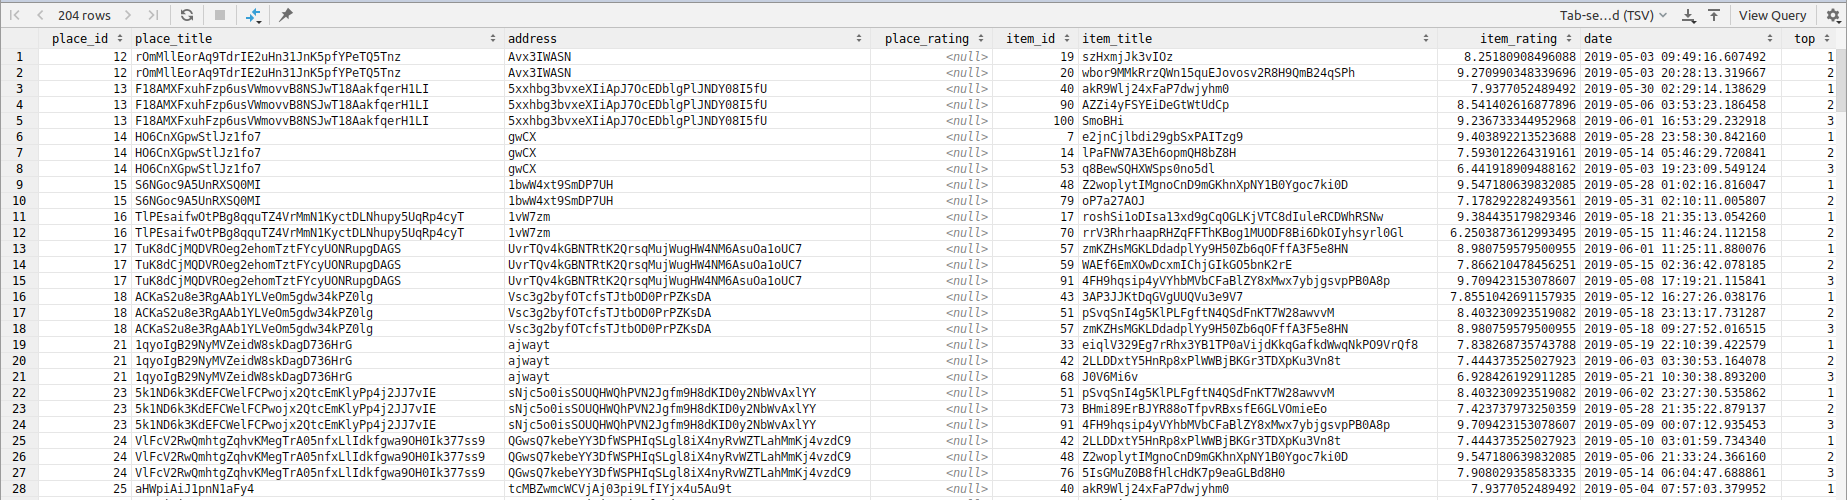
\includegraphics[scale=0.27]{ind_1}
		\caption{Результат работы} 
		\label{pic:ind_1} % название для ссылок внутри кода
	\end{center}
\end{figure}

\subsubsection{Индивидуальное задание №2}
Сначала формируется выборка из пар значений типа напиток -- количество компонентов.\\
\textit{(select d.drink\_id, count(d.drink\_id) components
	from drinks d
	join components\_drinks cd on d.drink\_id = cd.drink\_id
	group by d.drink\_id) sub}

Затем получившаяся выбока присоединяется к таблице напитков по равенству drink\_id.
Далее вычисляем среднее соличество компонентов среди всех напитков и ограничиваем выборку с помощью оператора where.
Наконец, группируем по drink\_id, components и сортируем по убыванию значения alcohol.

\lstinputlisting[
language=SQL,
caption={individual\_2.sql},
]{../../src/individual_2.sql}

\begin{lstlisting}[language=SQL, caption={План запроса}]
Sort  (cost=51.88..52.13 rows=102 width=97) (actual time=1.113..1.116 rows=50 loops=1)
Sort Key: d.alcohol DESC
Sort Method: quicksort  Memory: 34kB
InitPlan 1 (returns $0)
->  Aggregate  (cost=20.48..20.49 rows=1 width=32) (actual time=0.468..0.468 rows=1 loops=1)
->  HashAggregate  (cost=18.19..19.21 rows=102 width=12) (actual time=0.427..0.446 rows=102 loops=1)
Group Key: d_2.drink_id
->  Hash Join  (cost=4.29..15.40 rows=558 width=4) (actual time=0.046..0.262 rows=558 loops=1)
Hash Cond: (cd_1.drink_id = d_2.drink_id)
->  Seq Scan on components_drinks cd_1  (cost=0.00..9.58 rows=558 width=4) (actual time=0.006..0.066 rows=558 loops=1)
->  Hash  (cost=3.02..3.02 rows=102 width=4) (actual time=0.035..0.035 rows=102 loops=1)
Buckets: 1024  Batches: 1  Memory Usage: 12kB
->  Seq Scan on drinks d_2  (cost=0.00..3.02 rows=102 width=4) (actual time=0.004..0.018 rows=102 loops=1)
->  HashAggregate  (cost=26.96..27.98 rows=102 width=97) (actual time=1.049..1.065 rows=50 loops=1)
Group Key: d.drink_id, d_1.drink_id, (count(d_1.drink_id))
->  Hash Join  (cost=22.90..26.19 rows=102 width=81) (actual time=0.985..1.023 rows=50 loops=1)
Hash Cond: (d.drink_id = d_1.drink_id)
->  Seq Scan on drinks d  (cost=0.00..3.02 rows=102 width=69) (actual time=0.007..0.017 rows=102 loops=1)
->  Hash  (cost=21.62..21.62 rows=102 width=12) (actual time=0.971..0.971 rows=50 loops=1)
Buckets: 1024  Batches: 1  Memory Usage: 11kB
->  HashAggregate  (cost=19.58..20.60 rows=102 width=12) (actual time=0.920..0.960 rows=50 loops=1)
Group Key: d_1.drink_id
Filter: ((count(d_1.drink_id))::numeric > $0)
Rows Removed by Filter: 52
->  Hash Join  (cost=4.29..15.40 rows=558 width=4) (actual time=0.057..0.267 rows=558 loops=1)
Hash Cond: (cd.drink_id = d_1.drink_id)
->  Seq Scan on components_drinks cd  (cost=0.00..9.58 rows=558 width=4) (actual time=0.015..0.075 rows=558 loops=1)
->  Hash  (cost=3.02..3.02 rows=102 width=4) (actual time=0.038..0.038 rows=102 loops=1)
Buckets: 1024  Batches: 1  Memory Usage: 12kB
->  Seq Scan on drinks d_1  (cost=0.00..3.02 rows=102 width=4) (actual time=0.004..0.019 rows=102 loops=1)
Planning time: 0.496 ms
Execution time: 1.225 ms
\end{lstlisting}

\begin{figure}[H]
	\begin{center}
		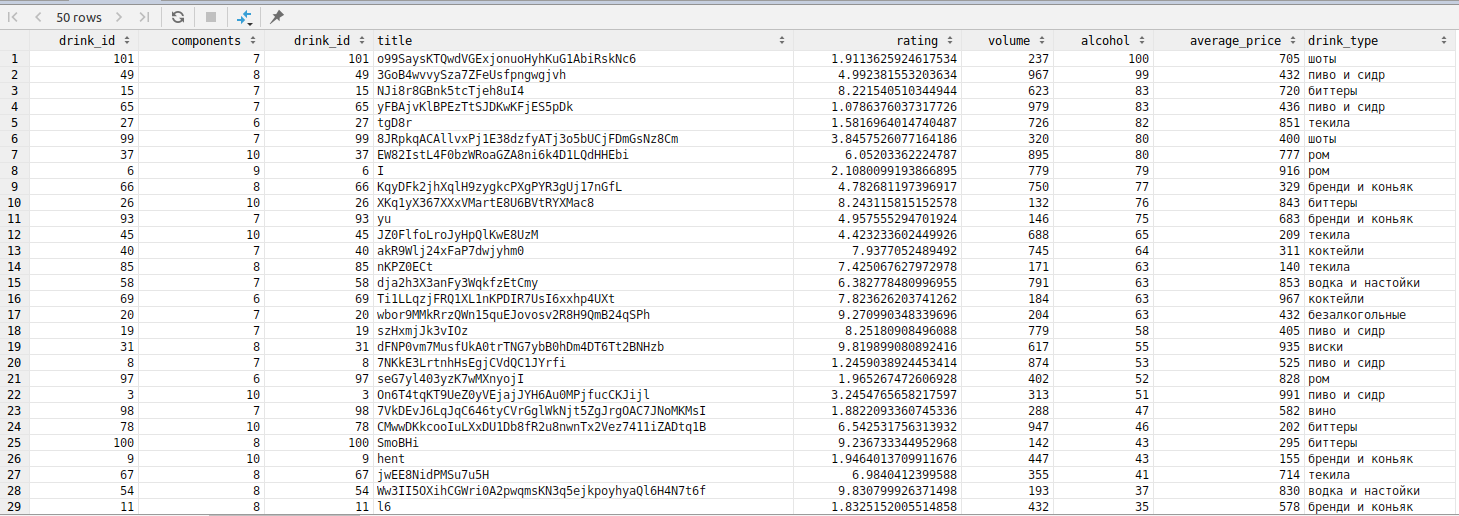
\includegraphics[scale=0.33]{ind_2}
		\caption{Результат работы} 
		\label{pic:ind_2} % название для ссылок внутри кода
	\end{center}
\end{figure}

\subsubsection{Индивидуальное задание №3}
С помощью оператора JOIN происходит объединение таблиц discounts и drinks по равенству поля drink\_type.
Таким образом, получем выборку из всевозможных акций на напитки.
Далее получивщуюся выбоку ограничиваем с помощью оператора where ... or ... or .. и требуемых условий.

\newpage
\lstinputlisting[
language=SQL,
caption={individual\_3.sql},
]{../../src/individual_3.sql}

\begin{lstlisting}[language=SQL, caption={План запроса}]
Sort  (cost=69.02..69.94 rows=365 width=135) (actual time=1.689..1.726 rows=420 loops=1)
Sort Key: drinks.alcohol DESC, drinks.average_price, drinks.volume DESC
Sort Method: quicksort  Memory: 136kB
InitPlan 1 (returns $0)
->  Aggregate  (cost=3.27..3.28 rows=1 width=8) (actual time=0.045..0.045 rows=1 loops=1)
->  Seq Scan on drinks drinks_1  (cost=0.00..3.02 rows=102 width=8) (actual time=0.004..0.020 rows=102 loops=1)
InitPlan 2 (returns $1)
->  Aggregate  (cost=3.27..3.28 rows=1 width=8) (actual time=0.041..0.041 rows=1 loops=1)
->  Seq Scan on drinks drinks_2  (cost=0.00..3.02 rows=102 width=8) (actual time=0.004..0.018 rows=102 loops=1)
InitPlan 3 (returns $2)
->  Aggregate  (cost=3.27..3.28 rows=1 width=8) (actual time=0.038..0.038 rows=1 loops=1)
->  Seq Scan on drinks drinks_3  (cost=0.00..3.02 rows=102 width=8) (actual time=0.004..0.017 rows=102 loops=1)
->  HashAggregate  (cost=39.99..43.64 rows=365 width=135) (actual time=1.016..1.239 rows=420 loops=1)
Group Key: discounts.discount_id, drinks.drink_id
->  Hash Join  (cost=3.83..38.16 rows=365 width=135) (actual time=0.203..0.709 rows=420 loops=1)
Hash Cond: (discounts.drink_type = drinks.drink_type)
->  Seq Scan on discounts  (cost=0.00..23.10 rows=1010 width=66) (actual time=0.011..0.172 rows=1009 loops=1)
->  Hash  (cost=3.79..3.79 rows=4 width=69) (actual time=0.164..0.164 rows=4 loops=1)
Buckets: 1024  Batches: 1  Memory Usage: 9kB
->  Seq Scan on drinks  (cost=0.00..3.79 rows=4 width=69) (actual time=0.138..0.161 rows=4 loops=1)
Filter: ((alcohol = $0) OR (average_price = $1) OR (volume = $2))
Rows Removed by Filter: 98
Planning time: 0.722 ms
Execution time: 1.853 ms
\end{lstlisting}

\begin{figure}[H]
	\begin{center}
		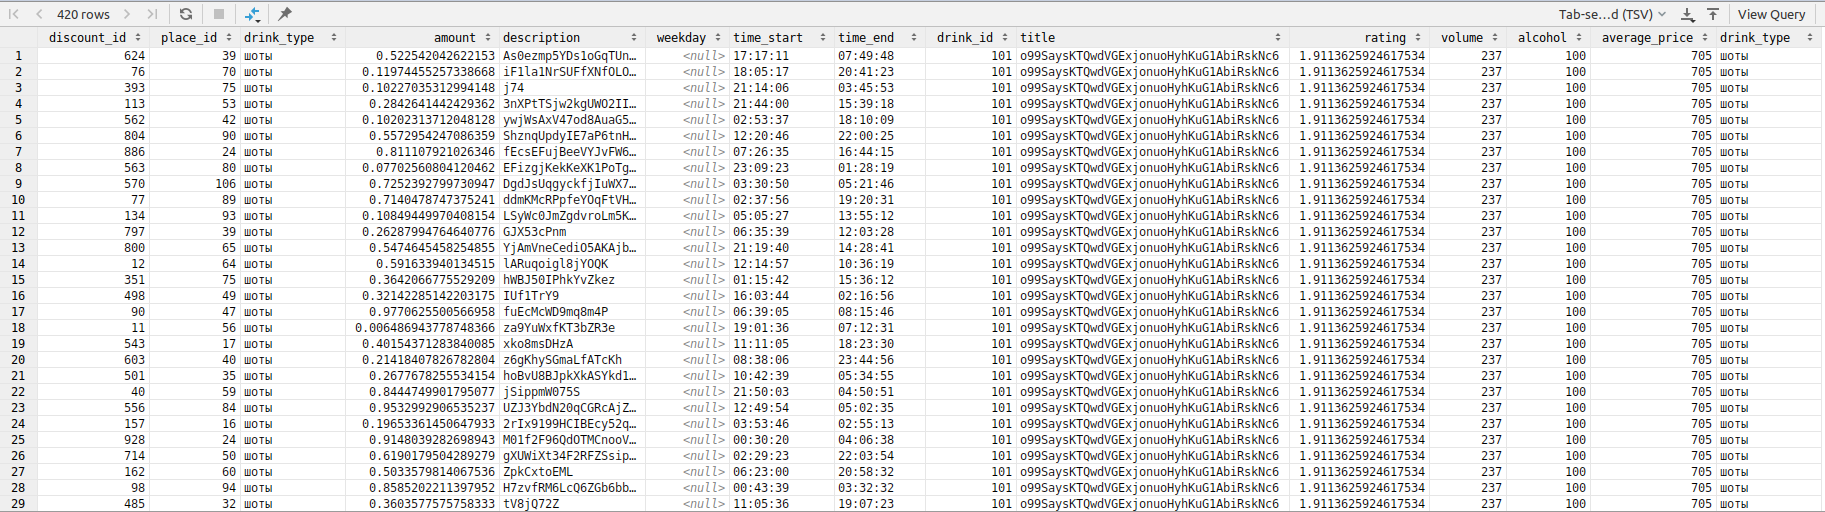
\includegraphics[scale=0.27]{ind_3}
		\caption{Результат работы} 
		\label{pic:ind_3} % название для ссылок внутри кода
	\end{center}
\end{figure}

\section{Выводы}
В ходе работы был изучен язык SQL-DML. Были созданы запросы к базе данных с
использованием операторов выбора SELECT, INSERT, DELETE и UPDATE.

Для извлечения записей из таблиц в SQL определен оператор SELECT. Этот оператор
возвращает ни одного, одно или множество строк, удовлетворяющих указанному условию и упорядоченных по заданному критерию. 

Оператор SELECT позволяет возвращать
не только множество значений полей, но и некоторые совокупные (агрегированные) характеристики, подсчитанные по всем или по указанным записям таблицы, например, SUM
(<имя поля>) – сумма всех значений данного поля. 

Также были рассмотрены и проанализированы планы запросов.
\end{document}
